\PassOptionsToPackage{table}{xcolor}
\documentclass[a1paper,portrait,american,fontscale=.4]{baposter}
\selectcolormodel{HTML}

\usepackage[utf8]{inputenc}
\usepackage[T1]{fontenc}
\usepackage{lipsum}
\usepackage{listings}
\usepackage{todo}
\usepackage{hyperref}
\usepackage{qrcode}
\usepackage{float}
\usepackage{algorithm}
\usepackage{algpseudocode}
\usepackage{multicol}
\usepackage{setspace}
\usepackage{bm}
\usepackage{marvosym}
\usepackage{amssymb}
\usepackage{tikz}
\usetikzlibrary{
    arrows,
    arrows.meta,
    backgrounds,
    calc,
    fit,
    chains,
    decorations,
    decorations.pathreplacing,
    matrix,
    positioning,
    scopes,
    shadows,
    shapes,
    shapes.multipart,
    shapes.arrows,
}

% TikZ coordinate system for whole page
\makeatletter
\def\parsecomma#1,#2\endparsecomma{\def\page@x{#1}\def\page@y{#2}}
\tikzdeclarecoordinatesystem{page}{
    \parsecomma#1\endparsecomma
    \pgfpointanchor{current page}{north east}
    % Save the upper right corner
    \pgf@xc=\pgf@x%
    \pgf@yc=\pgf@y%
    % save the lower left corner
    \pgfpointanchor{current page}{south west}
    \pgf@xb=\pgf@x%
    \pgf@yb=\pgf@y%
    % Transform to the correct placement
    \pgfmathparse{(\pgf@xc-\pgf@xb)/2.*\page@x+(\pgf@xc+\pgf@xb)/2.}
    \expandafter\pgf@x\expandafter=\pgfmathresult pt
    \pgfmathparse{(\pgf@yc-\pgf@yb)/2.*\page@y+(\pgf@yc+\pgf@yb)/2.}
    \expandafter\pgf@y\expandafter=\pgfmathresult pt
}
\makeatother

% vertical dots outside math mode
\makeatletter
\DeclareRobustCommand{\rvdots}{%
    \vbox{
        \baselineskip3\p@\lineskiplimit\z@
        \kern-\p@
        \hbox{.}\hbox{.}\hbox{.}
}}
\makeatother

\definecolor{MyColorOne}{HTML}{637462}
\definecolor{MyColorTwo}{HTML}{b7af8a}
\definecolor{MyColorThree}{HTML}{ccb15a}
\colorlet{MyBoxBG}{white!94!black}
\colorlet{MyLime}{lime!86!black}
\colorlet{MyOrange}{orange!92!black}
\colorlet{MyCyan}{cyan!70!blue}
\colorlet{MyTeal}{teal!70}
\colorlet{MyViolet}{violet!60}
%\colorlet{MyColorOne}{black}
%\colorlet{MyColorTwo}{black!30}

\tikzstyle{rect}=[draw,rectangle,thick,on chain,font=\tiny,inner sep=.5mm,minimum height=1.2em]
\tikzstyle{ssd}=[draw,rectangle,rounded corners,very thick,minimum width=3cm,minimum height=4cm]
\tikzstyle{ssd_screw}=[circle,fill=black!50!white,inner sep=0mm,minimum width=2mm]
\tikzstyle{memory}=[draw,rectangle,very thick,minimum width=18mm,minimum height=40mm]
\tikzstyle{file}=[draw,rectangle,minimum width=15mm,text width=15mm,minimum height=20mm,align=center]
\tikzstyle{fat_arrow}=[->,>={Triangle[length=7mm,width=10mm]},line width=6mm]
\tikzset{
    >=latex
}

\newcommand{\SSD}[3][]{%
    \node[ssd,#1] (#2) {#3};
    \node[below=1mm] at (#2.north) {\textbf{#2}};
    \node[ssd_screw,xshift=2mm,yshift=-2mm] at (#2.north west) {};
    \node[ssd_screw,xshift=-2mm,yshift=-2mm] at (#2.north east) {};
    \node[ssd_screw,xshift=2mm,yshift=2mm] at (#2.south west) {};
    \node[ssd_screw,xshift=-2mm,yshift=2mm] at (#2.south east) {};
}

\newcommand{\Memory}[3][]{%
    \node[memory,#1] (#2) {#3};
    \node[below=1mm,text width=15mm,align=center] at (#2.north) {\textbf{#2}};
}

\newcommand{\File}[2][]{%
    \node[file,#1] (#2)
        {%
            \ttfamily\tiny
            01000001010000\\
            11010011010010\\
            00000101001101\\
            00100101000111\\
            01001101010011\\
            11010001000010\\
            00000011001000\\
            11000000110001\\
            00111001\phantom{000000}\\

        };
    \node[above] at (#2.north) {\textbf{\footnotesize #2}};
}

\newcommand{\CPU}[3][]{%
    \node[draw,rectangle,very thick,minimum width=22mm,minimum height=22mm,#1] (#2) {};
    \node[draw,rectangle,very thick,rounded corners, minimum width=19mm,minimum height=19mm] at (#2) {#3};
    \node[below=3mm] at (#2.north) {\textbf{#2}};
}

\begin{document}
\begin{poster}{
        %----- Poster Settings -----------------------------------------------------------------------------------------
        background=none,
        columns=6,
        %----- Box Settings --------------------------------------------------------------------------------------------
        boxColorOne=MyBoxBG,
        boxshade=plain,
        headershade=shadeLR,
        headerColorOne=MyColorOne,
        headerColorTwo=MyColorTwo,
        textborder=roundedleft,
        borderColor=black,
        headerborder=open,
        headershape=roundedright,
        headerfont=\large\bfseries,
        headerFontColor=white!90!MyColorTwo,
        linewidth=0pt,
    }
    {}
    {
        \huge ACM~SIGMOD'19~Programming~Contest
    }
    {
        \vspace*{.5em}
        \emph{teamsic:}~Immanuel~L.~Haffner
        \qquad
        Advisor:~Jens~Dittrich
        \\[.5em]
        \large
        Big~Data~Analytics~Group, Saarland~Informatics~Campus
        \\[.5em]
        \url{bigdata.uni-saarland.de}
    }
    {
    }

    \headerbox{Task Description}{name=task,column=0,span=3}{
        \begin{center}
            \scalebox{.8}{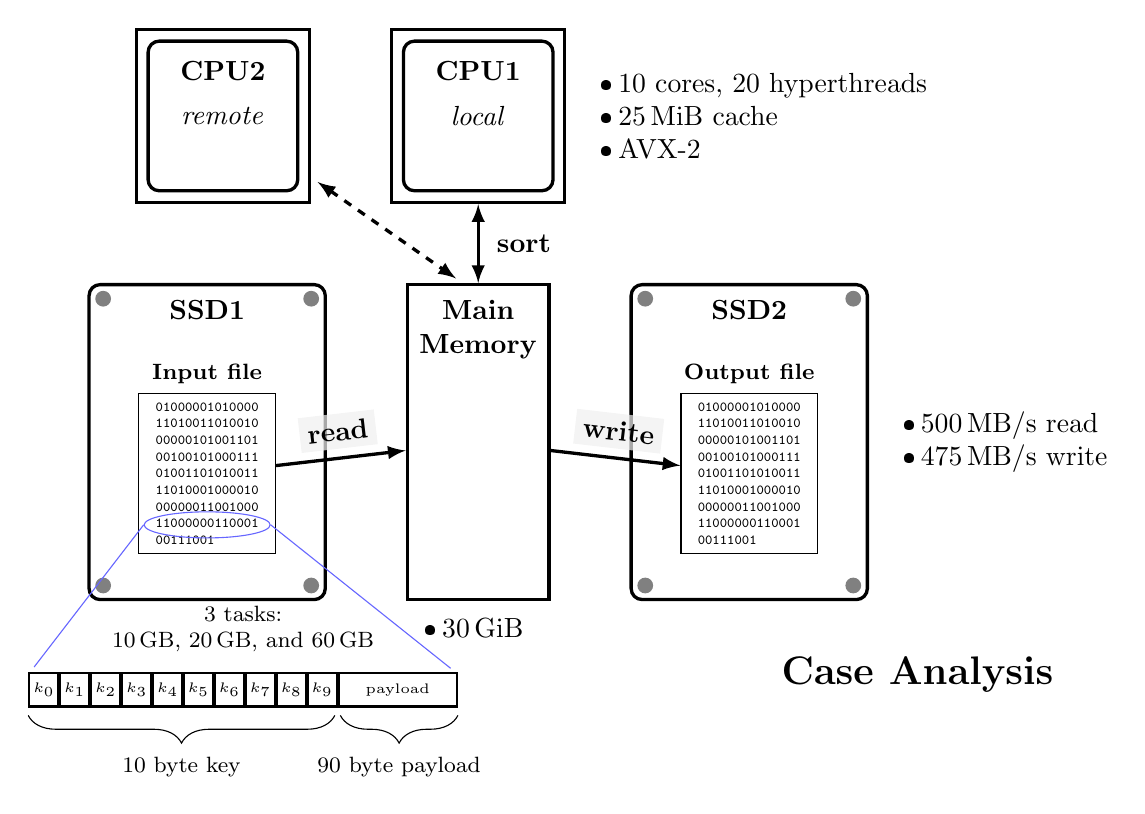
\begin{tikzpicture}[remember picture]
    % Hardware
    \SSD{SSD1}{};
    \Memory[right=10mm of SSD1]{Main Memory}{};
    \SSD[right=10mm of Main Memory]{SSD2}{};
    \File[anchor=south,above=6mm of SSD1.south]{Input file};
    \File[anchor=south,above=6mm of SSD2.south]{Output file};
    \draw[->,very thick] (Input file) to node[above=1mm,sloped,fill=MyBoxBG,inner sep=1mm,opacity=.7,text opacity=1] {\textbf{read}} (Main Memory);
    \draw[->,very thick] (Main Memory) to node[above=1mm,sloped,fill=MyBoxBG,inner sep=1mm,opacity=.7,text opacity=1] {\textbf{write}} (Output file);
    \CPU[above=of Main Memory]{CPU1}{\emph{local}};
    \draw[<->,very thick] (CPU1) -- node[right=1mm]{\textbf{sort}} (Main Memory.north);
    \CPU[left=of CPU1]{CPU2}{\emph{remote}};
    \draw[<->,very thick,dashed,shorten >=1mm,shorten <=1mm] (CPU2) -- ([xshift=-2mm]Main Memory.north);

    % Specification
    \node[right=3mm of CPU1,align=left]{%
        \textbullet\,10~cores, 20~hyperthreads
        \\
        \textbullet\,25\,MiB cache
        \\
        \textbullet\,AVX-2
    };

    \node[right=3mm of SSD2,align=left]{%
        \textbullet\,500\,MB/s read
        \\
        \textbullet\,475\,MB/s write
    };

    \node[below=1mm of Main Memory.south,align=left,anchor=north]{%
        \textbullet\,30\,GiB
    };

    \begin{scope}[start chain=going right,node distance=-.2\pgflinewidth,local bounding box=record]
        \node[rect,below left= 15mm and 10mm of Input file] (k0) {$k_0$};
        \node[rect] {$k_1$};
        \node[rect] {$k_2$};
        \node[rect] {$k_3$};
        \node[rect] {$k_4$};
        \node[rect] {$k_5$};
        \node[rect] {$k_6$};
        \node[rect] {$k_7$};
        \node[rect] {$k_8$};
        \node[rect] {$k_9$};
        \node[rect,minimum width=15mm] (payload) {payload};
    \end{scope}
    \draw[decorate,decoration={brace,mirror,amplitude=10pt,raise=1mm}]
    (k0.south west) -- node[below=5mm] {\footnotesize 10 byte key} ([xshift=-1pt]payload.south west);
    \draw[decorate,decoration={brace,mirror,amplitude=10pt,raise=1mm}]
    ([xshift=1pt]payload.south west) -- node[below=5mm] {\footnotesize 90 byte payload} (payload.south east);

    \node[ellipse,draw=blue!60,minimum height=2.6mm,minimum width=16mm] (zoom) at ([yshift=3.7mm] Input file.south) {};
    \draw[draw=blue!60,shorten >=1mm] (zoom.west) -- (record.north west);
    \draw[draw=blue!60,shorten >=1mm] (zoom.east) -- (record.north east);

    \node[above=1.5mm of record,align=center,font=\footnotesize] {3~tasks:\\10\,GB, 20\,GB, and 60\,GB};

    \node[align=left, right=40mm of record,yshift=2mm] (cases) {%
        \textbf{\Large Case Analysis}
    };
\end{tikzpicture}
}
        \end{center}
    }

    \headerbox{In-Memory Sorting}{name=inmemory,column=3,span=3}{
        \textbf{Algorithm:}
        \begin{algorithmic}[1]
            \footnotesize
            \setlength{\itemsep}{0em}
            \State predict record type (ASCII [32-126] or binary [0-255])
            \State estimate bucket sizes
            \State partition into 256 buckets
            \State sort each bucket with \emph{sicsort}
        \end{algorithmic}

        \begin{center}
            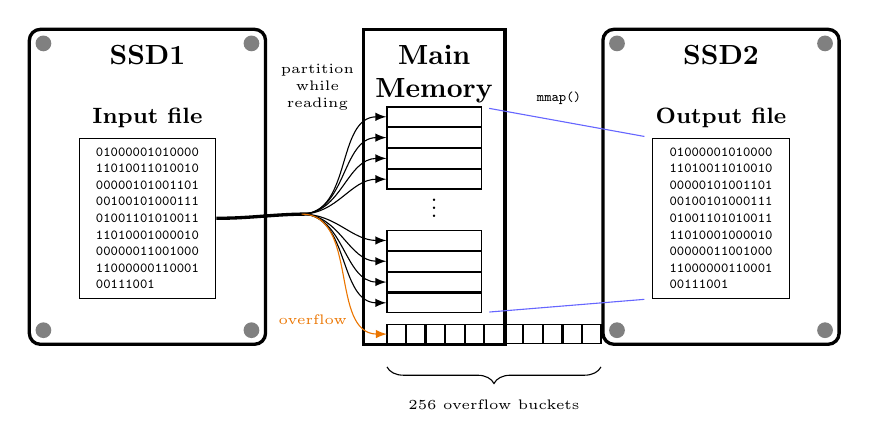
\begin{tikzpicture}[remember picture]
    \tikzstyle{part}=[on chain,draw,rectangle,minimum width=12mm,minimum height=2.5mm]

    % Hardware
    \SSD{SSD1}{};
    \Memory[right=12mm of SSD1]{Main Memory}{};
    \SSD[right=12mm of Main Memory]{SSD2}{};
    \File[anchor=south,above=6mm of SSD1.south]{Input file};
    \File[anchor=south,above=6mm of SSD2.south]{Output file};

    \begin{scope}[start chain=going below,node distance=0mm,local bounding box=array]
        \node[part,below=10mm of Main Memory.north] (a0) {};
        \node[part] (a1) {};
        \node[part] (a2) {};
        \node[part] (a3) {};
        \node[on chain,minimum height=5mm,font=\footnotesize] {\rvdots};
        \node[part] (a4) {};
        \node[part] (a5) {};
        \node[part] (a6) {};
        \node[part] (a7) {};
    \end{scope}

    \draw[draw=blue!60,shorten <= 1mm,shorten >=1mm] (array.north east) -- node[above=1mm,xshift=-1mm,font=\tiny] {\texttt{mmap()}} (Output file.north west);
    \draw[draw=blue!60,shorten <= 1mm,shorten >=1mm] (array.south east) -- (Output file.south west);

    \coordinate (split) at ($(Input file.east)!.5!(array.west)$);
    \draw[-,very thick,out=0,in=180] (Input file.east) to ([xshift=3pt]split);
    \draw[->,out=0,in=180] (split) to (a0);
    \draw[->,out=0,in=180] (split) to (a1);
    \draw[->,out=0,in=180] (split) to (a2);
    \draw[->,out=0,in=180] (split) to (a3);
    \draw[->,out=0,in=180] (split) to (a4);
    \draw[->,out=0,in=180] (split) to (a5);
    \draw[->,out=0,in=180] (split) to (a6);
    \draw[->,out=0,in=180] (split) to (a7);
    %\draw[->,out=0,in=180] (split) to (a8);
    \node[above=12mm of split,xshift=2mm,font=\tiny,align=center,text width=12mm] {partition while reading};

    \begin{scope}[start chain=going right,node distance=0mm,local bounding box=overflow]
        \node[on chain,draw,rectangle,minimum width=3pt,minimum height=5pt,anchor=north west,yshift=-4pt] at (a7.south west) {};
        \node[on chain,draw,rectangle,minimum width=3pt,minimum height=5pt] {};
        \node[on chain,draw,rectangle,minimum width=3pt,minimum height=5pt] {};
        \node[on chain,draw,rectangle,minimum width=3pt,minimum height=5pt] {};
        \node[on chain,draw,rectangle,minimum width=3pt,minimum height=5pt] {};
        \node[on chain,draw,rectangle,minimum width=3pt,minimum height=5pt] {};
        \node[on chain,draw,rectangle,minimum width=3pt,minimum height=5pt] {};
        \node[on chain,draw,rectangle,minimum width=3pt,minimum height=5pt] {};
        \node[on chain,draw,rectangle,minimum width=3pt,minimum height=5pt] {};
        \node[on chain,draw,rectangle,minimum width=3pt,minimum height=5pt] {};
        \node[on chain,draw,rectangle,minimum width=3pt,minimum height=5pt] {};
    \end{scope}
    \draw[->,MyOrange,out=0,in=180] (split) to node[font=\tiny,below=4mm,xshift=-4mm] {overflow} (overflow);

    \draw[decorate,decoration={brace,amplitude=6pt,raise=3mm}]
    (overflow.south east) -- node[below=6mm] {\tiny 256~overflow buckets} (overflow.south west);
\end{tikzpicture}

        \end{center}

        \vspace*{-5pt}
        \textbf{Tricks:}
        \vspace{-.5em}
        \begin{itemize}
            \setlength{\itemsep}{0em}
            \item avoid write to disk with \texttt{mmap()} \emph{\small\#thankskernel}
            \item keys are uniformly distributed; no skew
            \item partition into \texttt{mmap}'d output file while reading from disk:

            \begin{minipage}{.85\linewidth}
                \begin{algorithmic}\footnotesize
                    \State buckets $\gets$ \texttt{mmap(output file, ...)} \Comment{consecutive memory}
                    \For {%
                    \tikz[remember picture]{\coordinate (algo_start);}%
                    record $r$ \textbf{in} input file} \Comment{read from disk}
                        \State bucket $b \gets$ buckets[$r.k_0$] \Comment{initial partitioning}
                        \If {$b$ \textbf{is full}} \Comment{underestimated bucket size}
                            \State append $r$ to overflow bucket of $b$
                        \Else
                            \State append $r$ to $b$
                        \EndIf
                    \EndFor
                    \State \emph{patch\_overflow()}
                \end{algorithmic}
            \end{minipage}
        \end{itemize}
    }

    \headerbox{External Memory Sorting}{name=external,column=0,span=3,below=task}{
        \textbf{Algorithm:}
        \vskip 2pt
        \begin{minipage}{.8\linewidth}
        \begin{algorithmic}[1]
            \footnotesize
            \State $n \gets$ number of records that fit into main memory
            \State $s \gets$ read first $n$ records into main memory
            \State sort $s$ with \emph{sicsort} \Comment{in separate thread}
            \State partition remaining records into 256~files
            \For {every partition file $p$, sorted by size}
                \State sort $p$ with \emph{sicsort}
                \State merge $p$ with $s$ to output file on disk
            \EndFor
        \end{algorithmic}
        \end{minipage}

        \begin{center}
            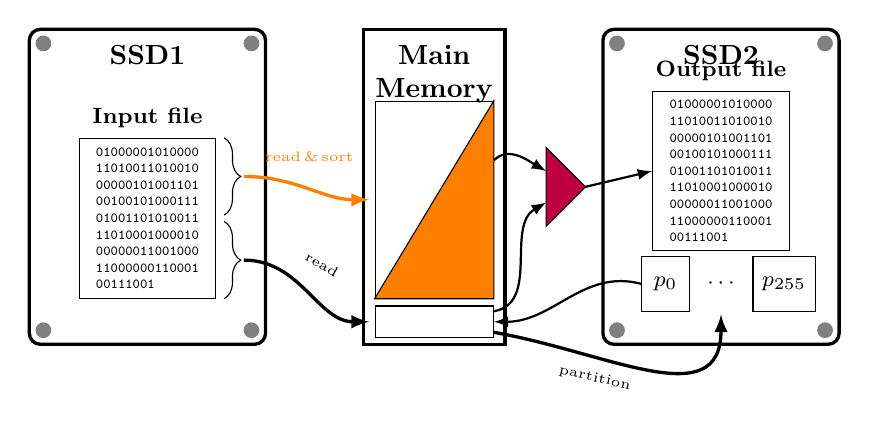
\begin{tikzpicture}[remember picture]
    % Hardware
    \SSD{SSD1}{};
    \Memory[right=12mm of SSD1]{Main Memory}{};
    \SSD[right=12mm of Main Memory]{SSD2}{};
    \File[anchor=south,above=6mm of SSD1.south]{Input file};
    \File[anchor=south,above=12mm of SSD2.south]{Output file};

    %\draw[->,very thick] (Input file) to node[above=1mm,sloped,fill=MyBoxBG,inner sep=1mm,opacity=.7,text opacity=1] {\textbf{read}} (Main Memory);
    %\draw[->,very thick] (Main Memory) to node[above=1mm,sloped,fill=MyBoxBG,inner sep=1mm,opacity=.7,text opacity=1] {\textbf{write}} (Output file);

    \draw[decorate,decoration={brace,amplitude=6pt,raise=1mm}]
    (Input file.north east) -- coordinate[xshift=10pt] (to_sort) ($(Input file.north east)!.48!(Input file.south east)$);
    \draw[decorate,decoration={brace,amplitude=6pt,raise=1mm}]
    ($(Input file.north east)!.52!(Input file.south east)$) -- coordinate[xshift=10pt] (to_partition) (Input file.south east);

    \node[draw,rectangle,minimum width=15mm,minimum height=25mm,above=6mm of Main Memory.south] (sorted) {};
    \draw[fill=orange] (sorted.south west) -- (sorted.south east) -- (sorted.north east) -- cycle;

    \node[draw,rectangle,minimum width=15mm,minimum height=4mm,above=1mm of Main Memory.south] (buffer) {};

    \draw[->,orange,very thick,shorten >=2pt,out=0,in=180] (to_sort) to node[above=2mm,font=\tiny] {read\,\&\,sort} (sorted.west);
    \draw[->,very thick,shorten >=2pt,out=0,in=180] (to_partition) to node[above=2mm,rotate=-30,xshift=2pt,font=\tiny] {read} (buffer.west);

    \node[minimum width=5mm,font=\footnotesize,above=6mm of SSD2.south] (partitions) {$\cdots$};
    \node[draw,rectangle,minimum height=7mm,minimum width=6mm,font=\footnotesize,left=1mm of partitions] (p0) {$p_0$};
    \node[draw,rectangle,minimum height=7mm,minimum width=6mm,font=\footnotesize,right=1mm of partitions] (p2) {$p_{255}$};

    \draw[->,very thick,shorten >=2mm,out=-10,in=270,looseness=1.3] (buffer) to node[below left=1mm,rotate=-13,font=\tiny] {partition} (partitions.south);
    \draw[->,thick,out=165,in=0] (p0.west) to (buffer);

    \coordinate[right=5mm of Main Memory] (merge);

    \draw[fill=purple] ($(merge)+(0,.5)$) -- ($(merge)+(.5,0)$) -- ($(merge)-(0,.5)$) -- cycle;
    \draw[->,thick,out=10,in=210] (buffer) to ($(merge)-(0,.2)$);
    \draw[->,thick,in=150] ($(sorted.east)+(0,.5)$) to ($(merge)+(0,.2)$);
    \draw[->,thick] ($(merge)+(.5,0)$) to (Output file.west);
\end{tikzpicture}

        \end{center}

        \vspace{-6mm}
        \begin{center}
            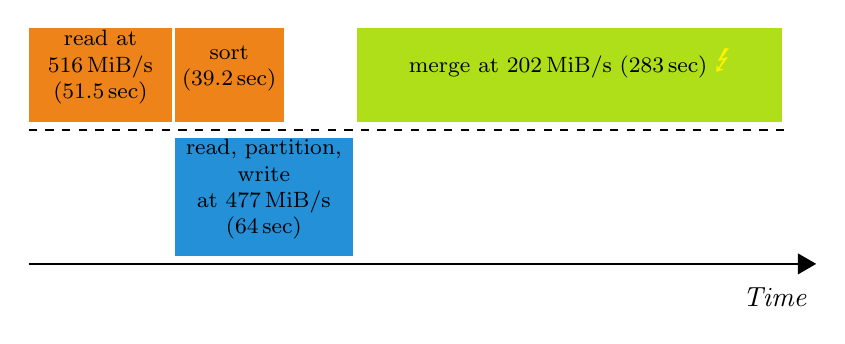
\begin{tikzpicture}
    \tikzstyle{box}=[rectangle,align=center,font=\footnotesize,inner sep=0pt]
    \draw[-triangle 60,thick] (0,0) -- (10,0);
    \draw[dashed] (0,1.7) -- (9.6,1.7);
    \node[below=.5em,anchor=north east,font=\itshape] at (10,0) {Time};

    \node[box,fill=MyOrange!90,fit={(0,3.0)(1.82,1.8)}] {read at 516\,MiB/s\\(51.5\,sec)};
    \node[box,fill=MyOrange!90,fit={(1.82,3.0)(3.2,1.8)},xshift=1pt] {sort\\(39.2\,sec)};
    \node[box,fill=MyCyan!90,fit={(1.82,0.1)(4.08,1.6)},xshift=1pt] {read, partition, write at~477\,MiB/s\\(64\,sec)};
    \node[box,fill=MyLime!90,fit={(4.1,3.0)(9.5,1.8)},xshift=2pt] {merge at~202\,MiB/s (283\,sec)~\textcolor{yellow}{\large\Lightning}};
\end{tikzpicture}

        \end{center}
    }

    \headerbox{Third-Party Libraries}{name=libs,column=0,span=3,below=external}{
        \begin{itemize}
            \setlength{\itemsep}{0em}
            \item Agner Fog's \texttt{asmlib} {\footnotesize (for \texttt{memcmp()})}
            \item CTPL: Modern and Efficient C\texttt{++} Thread Pool Library {\footnotesize (not in final submission)}
            \item Intel Processor Counter Monitor (PCM) {\footnotesize (not in final submission)}
        \end{itemize}
    }

    \headerbox{Sorting Algorithm \emph{sicsort}}{name=algo,column=3,span=3,below=inmemory}{
        \textbf{Algorithm:}
        \begin{algorithmic}[1]
            \footnotesize
            \State compute histogram
            \State compute partition boundaries
            \For{every record $r$}
                \If {$r$ in destination partition}
                    \State proceed to next record
                \Else
                    \State $p \gets$ destination partition of $r$
                    \State swap $r$ with unpartitioned record of $p$
                \EndIf
            \EndFor
        \end{algorithmic}

        \vspace*{-5mm}
        \begin{center}
            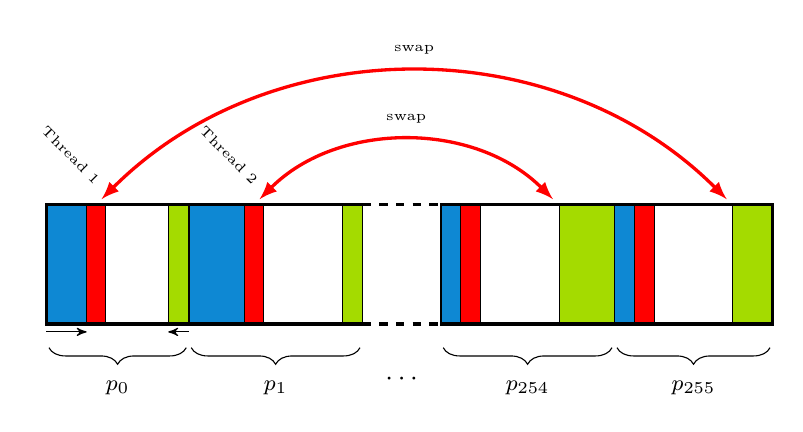
\begin{tikzpicture}[
    part/.style={on chain,draw,minimum width=2.5mm,minimum height=15mm,font=\tiny},
    arr/.style={<->,very thick,shorten <=1mm,shorten >=1mm,out=45,in=135,red},
    node distance=-\pgflinewidth
    ]
    \begin{scope}[start chain=going right,local bounding box=array]
        \node[part,fill=MyCyan,minimum width=5mm] (head1) {};
        \node[part,fill=red] (curr1) {};
        \node[part,minimum width=8mm] {};
        \node[part,fill=MyLime] (tail1) {};

        \node[part,fill=MyCyan,xshift=.5\pgflinewidth,minimum width=7mm] (head2) {};
        \node[part,fill=red] (curr2) {};
        \node[part,minimum width=10mm] {};
        \node[part,fill=MyLime] (tail2) {};

        \node[on chain,minimum width=10mm] {};

        \node[part,fill=MyCyan] (head3) {};
        \node[part,fill=red] (curr3) {};
        \node[part,minimum width=10mm] {};
        \node[part,fill=MyLime,minimum width=7mm] (tail3) {};

        \node[part,fill=MyCyan,xshift=.5\pgflinewidth] (head4) {};
        \node[part,fill=red] (curr4) {};
        \node[part,minimum width=10mm] {};
        \node[part,fill=MyLime,minimum width=5mm] (tail4) {};
    \end{scope}

    \draw[very thick] (tail2.north east) -- (head1.north west) -- (head1.south west) -- (tail2.south east);
    \draw[very thick,dashed] (tail2.north east) -- (head3.north west);
    \draw[very thick,dashed] (tail2.south east) -- (head3.south west);
    \draw[very thick] (head3.north west) -- (tail4.north east) -- (tail4.south east) -- (head3.south west);

    \draw[arr] (curr1.north) to node[above=1mm,font=\tiny,black] {swap} (tail4.north west);
    \draw[arr] (curr2.north) to node[above=1mm,font=\tiny,black] {swap} (tail3.north west);

    \draw[->,>=stealth'] ([yshift=-1mm]head1.south west) to ([yshift=-1mm]head1.south east);
    \draw[<-,>=stealth'] ([yshift=-1mm]tail1.south west) to ([yshift=-1mm]tail1.south east);

    \draw[decorate,decoration={brace,amplitude=6pt,raise=3mm}] ([xshift=-1pt]tail1.south east) -- node[below=6mm,font=\footnotesize] {$p_0$} ([xshift=1pt]head1.south west);
    \draw[decorate,decoration={brace,amplitude=6pt,raise=3mm}] ([xshift=-1pt]tail2.south east) -- node[below=6mm,font=\footnotesize] {$p_1$} ([xshift=1pt]head2.south west);
    \draw[decorate,decoration={brace,amplitude=6pt,raise=3mm}] ([xshift=-1pt]tail3.south east) -- node[below=6mm,font=\footnotesize] {$p_{254}$} ([xshift=1pt]head3.south west);
    \draw[decorate,decoration={brace,amplitude=6pt,raise=3mm}] ([xshift=-1pt]tail4.south east) -- node[below=6mm,font=\footnotesize] {$p_{255}$} ([xshift=1pt]head4.south west);
    \node[below=5mm] at ($(tail2.south east)!.5!(head3.south west)$) {$\cdots$};

    \node[font=\tiny,rotate=-45,anchor=east,above left=2pt of curr1.north,yshift=1pt] (thread1) {Thread 1};
    \node[font=\tiny,rotate=-45,anchor=east,above left=2pt of curr2.north,yshift=1pt] (thread2) {Thread 2};
\end{tikzpicture}

        \end{center}

        \vspace*{-2mm}
        \textbf{Details:}
        \vspace{-.5em}
        \begin{itemize}
            \setlength{\itemsep}{0em}
            \item based on \emph{American Flag Sort}, an in-place radix sort
            \item extended with parallel partitioning (see figure above)
            \item parallelize recursion into partition
            \item fall back to \texttt{std::sort()} on recursion if number of records is small (i.e.\ \emph{introsort}
                with fall back to \emph{insertion sort})
            \item atomic counters for head and tail of each partition
            \item avoid cache contention
                \vspace{-.5em}
                \begin{itemize}
                    \setlength{\itemsep}{0em}
                    \item pad counters to 64\,Bytes $\Rightarrow$ one cache line per counter
                    \item with $256$ partitions requires exactly 32\,KiB cache (L1D)
                \end{itemize}
        \end{itemize}%
        \vspace*{-5.8pt}
    }

    \headerbox{Ranking}{name=eval,column=0,span=3,below=libs}{
        \begin{itemize}
            \setlength{\itemsep}{0em}
            \item preliminary third place
            \item first in \emph{Small} (10\,GB) with~17\,\% margin to second
            \item first in \emph{Medium} (20\,GB) with~12\,\% margin to second
            \item fifth in \emph{Large} (60\,GB) with~15\,\% margin to best
        \end{itemize}
    }
\end{poster}

\vspace*{-6em}
\begin{tikzpicture}[overlay,remember picture]
    \coordinate (arr_task_to_inmemory) at (page cs:0,.34);
    \coordinate (arr_task_to_external) at (page cs:-.12,.265);
    \coordinate (arr_extern_uses) at (page cs:0,-.36);
    \coordinate (arr_inmemory_uses) at (page cs:.75,-.03);

    % < 30 GiB
    \draw[fat_arrow,draw=MyColorOne] ([xshift=-8mm]arr_task_to_inmemory) to
        node[white,font=\ttfamily\footnotesize] {<\,30\,GiB}
        ([xshift=8mm]arr_task_to_inmemory);
    % ≥ 30 GiB
    \draw[fat_arrow,draw=MyColorOne] ([yshift=8mm]arr_task_to_external) to
        node[white,font=\ttfamily\footnotesize,rotate=90] {$\bm\geqslant$\,30\,GiB}
        ([yshift=-8mm]arr_task_to_external);

    % extern uses algo
    \draw[fat_arrow,draw=MyColorOne] ([xshift=-8mm]arr_extern_uses) to
        node[white,font=\small] {uses}
        ([xshift=8mm]arr_extern_uses);
    % in-memory uses algo
    \draw[fat_arrow,draw=MyColorOne] ([yshift=8mm]arr_inmemory_uses) to
        node[white,font=\small,rotate=90] {uses}
        ([yshift=-8mm]arr_inmemory_uses);

    \node[anchor=north east,align=right,xshift=-4.5mm,yshift=-3.5mm] at (page cs:1,1) {%
        \qrcode[height=20mm]{https://git.io/fjazH}
        \\[.5em]
        \hfill\mbox{\small\url{git.io/fjazH}}
    };
\end{tikzpicture}

\clearpage
\todos

\end{document}
